%!TEX root = ../dissertation.tex
\begin{savequote}[75mm]
This is some random quote to start off the chapter.
\qauthor{Firstname lastname}
\end{savequote}

\chapter{Electronic cooling mechanisms in graphene}
\label{ch:electronic_cooling}
\newthought{Charge carriers in conductors} exchange energy with the environment in many ways. If an electronic system is directly heated --- whether it be by Joule heating, optical pumping, and any other direct energy transfer --- the mechanisms with which the system cools can be quite diverse. In mesoscopic samples there are typically three cooling mechanisms one has to consider. First, if the material is electrically connected to a thermal bath, such as macroscopic electrodes, then hot electrons can diffuse out and cold electrons can diffuse in; this diffusion is often referred to as Wiedemann-Franz cooling and is the dominate thermal transport mechanism in metals at low temperature~\cite{ashcroft_solid_1976, kittel_introduction_2004}. Secondly, hot electrons can transfer energy directly to the lattice by coupling to acoustic and optical phonon modes in the graphene itself or the nearby substrate~\cite{??}. Thirdly, electrons are charged and can therefore radiatively cool; this radiation is often in the form of Johnson noise and, although often negligible even at cryogenic temperature, can be the dominate cooling mechanism in ultra-sensitive bolometers~\cite{prober, mckitterick??}.


\section{Wiedemann-Franz}
\newthought{If a material hosts mobile charge carriers}, at a fixed temperature, each quasiparticle can transport a quantized amount of thermal energy and a quantized charge through the system; it then stands to reason the electronic thermal conductance must be related to the electrical conductivity. First observed at room temperature in 1853 by Wiedemann and Franz~\cite{franz_ueber_1853},  the thermal conductivity, $\kappa$, of metals is directly proportional to the electrical conductivity, $\sigma$, at room temperature. Twenty years later, Lorenz expanded upon the idea and showed the ratio of the thermal conductivity to the product of the electrical conductivity and temperature, $T$, was a constant~\cite{lorenz_bestimmung_1872}, $\sL$.
\begin{equation}\label{eq:WF}
\frac{\kappa}{\sigma T} = \sL
\end{equation}
Eq.~\ref{eq:WF} is now known as the Wiedemann-Franz law (WFL) where $\sL$ is the Lorenz ratio. Data showing experimentally measured Lorenz numbers for various metals and semi conductors as a function of conductivity and carrier concentration is shown in fig.~\ref{fig:WF_in_metals}.
\begin{figure}
\centering
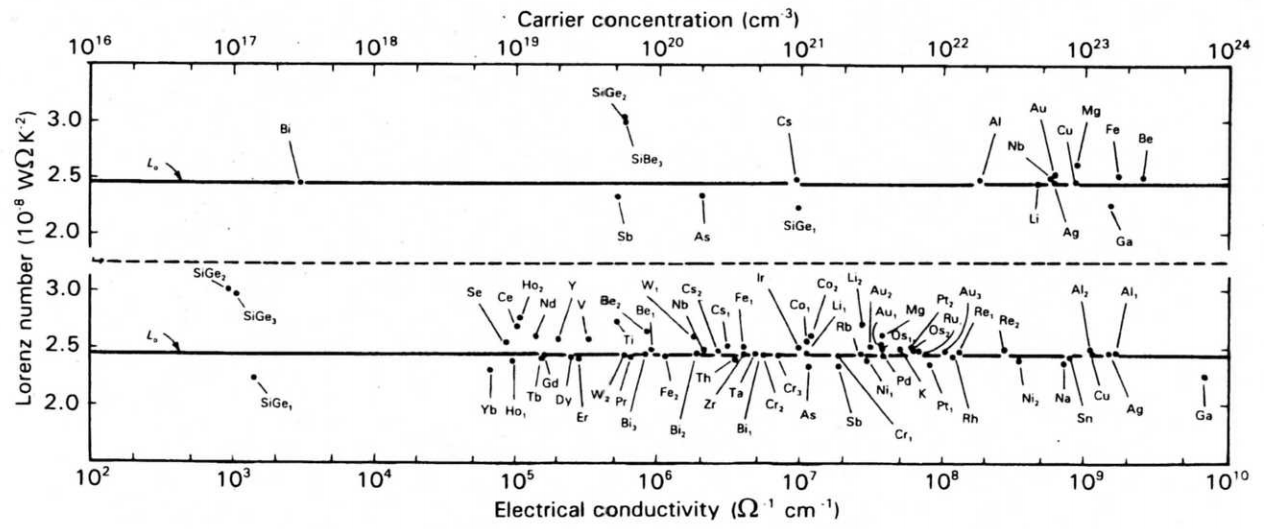
\includegraphics[width=\textwidth]{figures/electronic_cooling/WF_in_metals.png}
\caption{Experimental Lorentz number of elemental metals and degenerate semiconductors at low temperature. Taken from ref~\cite{kumar_experimental_1993}. \textit{reprinted with permission, Springer, license number 4067330556225}}
\label{fig:WF_in_metals}
\end{figure}
The quantitative value for $\sL$ can be approximated under the Drude model~\cite{ashcroft_solid_1976} but it was not until Sommerfeld in 1927 that a full derivation using Fermi-Dirac statistics was presented~\cite{sommerfeld}. Under the assumptions of a degenerate Fermi gas and only elastic collisions, the theoretical value of the Lorentz number was shown to be:
\begin{equation}
\sL = \sL_0 \equiv \frac{\pi^2}{3}\frac{k_B^2}{e^2} \approx 2.44\times10^{-8}~\Watt\Omega/K^2
\end{equation}
The requirement that quasiparticles only scatter elastically leads the value of $\sL$ to deviate from $\sL_0$ in the presence of strong electron-electron scattering and inelastic electron-phonon scattering. WF conduction can be suppressed with the use of superconducting leads~\cite{mckitterick_prospects_2015}.

\subsection{Linearization}
To understand the behavior of devices under low energy excitations, it is useful to linearize the WFL. In the linear response regime the temperature variations across a device are small compared to the absolute temperature scale of the problem, $T_b$. For a uniform two-dimension device connecting two thermal baths with temperatures $T_b \pm\Delta T/2$, the steady state thermal power transported via the WFL is given by:
\begin{equation}\label{eq:QWF}
\Qdot_{WF} = \left(\frac{W\sigma}{L}\right)\sL T_b~\Delta T = \frac{\sL T_b}{R}\Delta T
\end{equation}
where W and L are the sample width and length, respectively, and R is the two-terminal electrical resistance
\subsection{Hot-electron shot noise}
A common way to develop a temperature gradient is via Joule heating where the electron temperature is raised with reference to the cold electrodes held at $T_b$. In the case of only WF conduction --- i.e. no alternative cooling pathways such as phonons --- the temperature rise in the high current regime scales linear in the current producing noise very similar to the shot noise seen in vacuum tubes. This well known effect is termed ``hot-electron shot noise"~\cite{steinbach_observation_1996,blanter_shot_2000,de_jong_semiclassical_1996} and can be seen as the limit of the WFL with $T_e >> T_b$.
\begin{equation}\label{eq:hot_electron_Q}
\Qdot \approx \frac{\alpha\sl}{R}T_e^2
\end{equation}
where $\alpha$ is a constant related to the temperature profile in the device. If we set the power dissipated to be proportional to the current squared, such that $\Qdot = I^2R$, we find:
\begin{equation}\label{eq:hot_electron_Te}
\langle T_e\rangle \approx \frac{R}{\sqrt{\alpha\sL}}~I
\end{equation}
Solving for the temperature profile and the noise produced, eq.~\ref{eq:hot_electron_Te} reduces to~\cite{martinez??}:
\begin{equation}\label{eq:hot_electron_I}
S_I = \frac{\sqrt{3}}{4}2e~I
\end{equation}
Eq.\ref{eq:hot_electron_I} has the same form as shot noise with Fano factor of $\sqrt{3}/4$.

\section{Electron-Phonon coupling}
At higher temperatures, the cooling of hot electrons is dominated by coupling to acoustic and optical phonons in the hexangonal lattice as well as the nearby substrate~\cite{viljas_electron-phonon_2010,bistritzer_electronic_2009}. In many experiments involving optical heating or Joule heating, a quasi-equilibrium can be formed where the electron temperature and the lattice temperature can be different. In the particular case of monolayer graphene this is especially true as the high phonon conductivity and relatively weak electron-phonon coupling can result in a lattice temperature that is well sunk to the thermal bath, $T_b$, but an elevated electron temperature, $T_e$. The interaction between this relativistic fermionic and bosonic system in graphene is quite rich with even the power law for the temperature dependence varying depending on the Fermi level, device disorder, and bias voltage. A general form for the heat transfer between the two systems can written as:
\begin{equation}\label{eq:Qelph}
\Qdot_{e-ph}=\mathrm{A}~\Sigma_{e-ph}\left( T_e^{~\de} - T_b^{~\de} \right)
\end{equation}
where $\mathrm{A}$ is the area of the device, $\Sigma_{e-ph}$ is a coupling constant, and $\de$ is the is the power law exponent. Depending on the mechanism $\de$ is typically $3$~\cite{song_disorder-assisted_2012, chen_electron-phonon_2012} in disordered samples,  or $4--5$ in clean devices~\cite{viljas_electron-phonon_2010, bistritzer_electronic_2009}. These relatively high power laws result in phonons dominating at high temperature but becoming negligible when cold.
\subsection{Linearization}
To find the linear response behavior ($\Delta T \ll T_b$) we can Taylor expand to first order for $T_e\approx T_b$ to find:
\begin{equation}\label{eq:Qelph_linear}
\Qdot_{e-ph} \approx \mathrm{A}~\de~\Sigma_{e-ph}T_b^{~\de-1}~\Delta T
\end{equation}
Eq.~\ref{eq:Qelph_linear} can be compared to eq.~\ref{eq:QWF}. First we see that while both cooling mechanisms scale as the device width, they have inverse dependences on the device length and as such the bath temperature at which one mechanism will dominate over the other is geometry dependent.

The literature on electron-phonon coupling in graphene is vast~\cite{??,shaffique,flexure,sohier_phonon-limited_2014}. I present here a simplified review of the main mechanisms relevant to the experiments presented here.

\subsection{Bloch-Gr{\"u}neisen temperature}
In most three-dimensional metals, where the Fermi surface is large, the characteristic temperature scale for phonon dynamics is given by the Debye temperature. However, in semiconductors and semimetals the Fermi surface can be substantially smaller than the Brillouin zone and a second temperature scale governs the scattering of electrons and phonons. The Bloch-Gr{\"u}neisen temperature, $T_{BG}$, is the temperature at which the most energetic phonons have a typical momentum equal to the Fermi momentum\cite{bloch_zum_1930, gruneisen_abhangigkeit_1933}.
\begin{equation}\label{eq:TBG}
T_{BG} = 2\hbar v_sk_F/k_B
\end{equation}
Above this temperature, momentum conservation dictates that only a fraction of the available phonon modes can scatter electrons; the largest momentum change an electron can experience is $2k_F$ --- a complete backscatter --- and as such, only phonons with momentum equal to or less than $2k_F$ can participate in scattering processes. This has been shown in $GaAs$ based 2D electron systems~\cite{stormer_observation_1990} and in graphene~\cite{efetov_controlling_2010} where $T_{BG}$ can be controlled by tuning the Fermi level using an electrostatic gate.

\subsection{Acoustic phonons}
In typical metals at low temperature, the dominate phonon modes in the system are acoustic~\cite{ashcroft_solid_1976}\footnote{The optical phonon branch has finite energy at $k=0$ and thus at low enough temperatures these modes are frozen out}. In graphene, however, energy transfer between electrons and these acoustic phonons (AP) is limited by the mismatch between the Fermi velocity, $v_F$, and the sound speed in the material, $v_s$. Energy and momentum conservation limit the energy each phonon collision can remove from the electronic system resulting a maximal energy transfer of $2\hbar v_sk_F$. Nevertheless, experiments have shown that the electronic cooling in many graphene devices at low temperatures can be dominated by AP scattering~\cite{fong_measurement_2013, betz_supercollision_2013, graham_photocurrent_2013} .

Theoretical predictions for the the power law $\de$ and the coupling constant $\Sigma_{e-ph}$ have been shown to depend upon the device temperature and the amount of disorder. In the dirty limit, the energy and momentum conservation discussed above can be circumvented by disorder-assisted collisions called ``supercollisions" resulting in a  power law $\de=3$~\cite{song_disorder-assisted_2012}. In the clean limit at low temperature, Kubakaddi~\cite{kubakaddi_interaction_2009} showed $\de = 4$ with a coupling constant:
\begin{equation}\label{eq:Sigma_e-ac}
\Sigma_{e-ap}=\frac{\pi^2\mathcal{D}^2\lvert\m\rvert k_B^4}{15\p\hbar^5v_F^3v_s^3}
\end{equation}
where $\mathcal{D}$ is the deformation potential, $\m$ is the chemical potential, and $\p$ is the mass density of the lattice.
Eq.~\ref{eq:Sigma_e-ac} was reproduced by
Viljas et al.~\cite{viljas_electron-phonon_2010} and extended to high temperature where it was found $\de$ approaches $5$. The transisiton from these two regimes is shown in fig.~\ref{fig:viljas2010}.
\begin{figure}
\centering
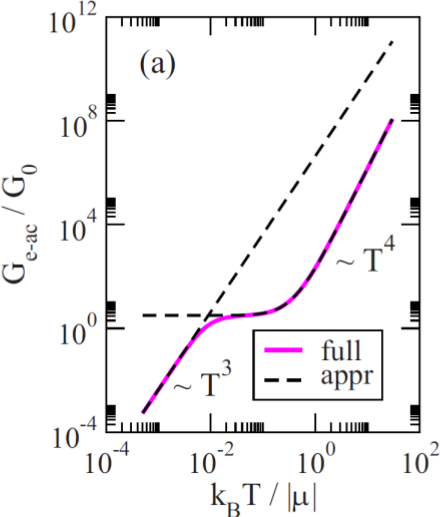
\includegraphics[width = 70mm]{figures/electronic_cooling/Viljas2010_conduction.png}
\caption{
Reprinted figure with permission from
ref.~\cite{viljas_electron-phonon_2010} by the American Physical Society license number: 4077361227141.}
\label{fig:viljas2010}
\end{figure}


\subsection{Optical phonons}

Although the energies associated with optical phonons in graphene are quite large compared to the thermal energies in typical experiments, each collision can remove a significant amount of energy from the electronic system. Bistritzer et al.~\cite{bistritzer_electronic_2009} showed that at sufficiently high temperatures even the ${\sim200}~meV$ intrinsic can dominate electronic cooling in suspended samples. For encapsulated devices, remote phonons in the boron-nitride have been shown to have a surprisingly significant effect both theroetically~\cite{viljas_electron-phonon_2010, bistritzer_electronic_2009, low_cooling_2012} and experimentally~\cite{tielrooij_out--plane_2017}. At higher temperature $\left( \gtrsim 270~K\right)$, Sohier et al.~\cite{sohier_phonon-limited_2014} showed that despite the relatively low occupancy, graphene intrinsic optical phonons can have a more pronounced effect on the electrical resistance than acoustic phonons.

\section{Photon cooling}
For a device coupled to a microwave circuit, energy is radiated via photons over the measurement bandwidth~\cite{schmidt_photon-mediated_2004, mckitterick_prospects_2015}. This is equivalent to 1D blackbody radiation and is the noise which is measured in Johnson noise thermometry. The power transferred is given by eq.~\ref{eq:NyquistPower} which is negligible compared to Wiedemann-Franz and phonon cooling for the temperatures and bandwidths covered in this thesis. However, for devices at low temperature with superconducting leads this can become a significant source of thermalization~\cite{mckitterick_prospects_2015}.

\section{Thermal Network}
In general, when heat is injected into the electronic system of graphene, each of the mechanisms described above plays a role in thermalizing the system to an external bath. For the devices and experimental parameters used in this thesis, a simplified thermal model can be used, illustrated in fig.~\ref{fig:thermal_diagram}.
\begin{figure}
\centering
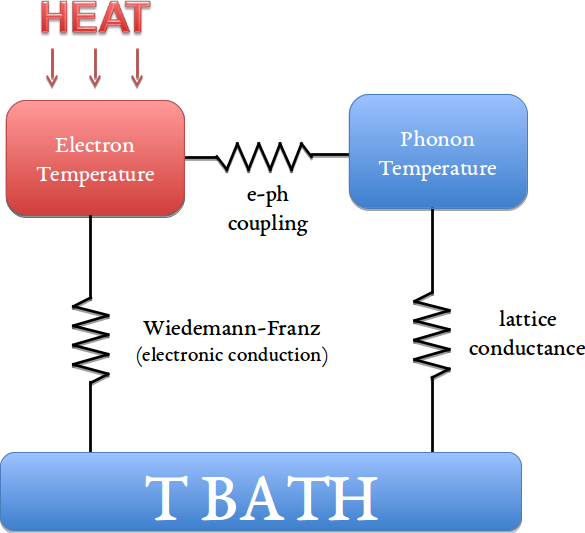
\includegraphics[width = 90mm]{figures/electronic_cooling/Thermal_diagram.png}
\caption{A thermal model of the electronic cooling pathways in graphene. Heat injected into the electronic system can flow directly to the bath via Wiedemann-Franz conduction, or to the lattice via electron-phonon coupling. The lattice and the bath are connected via the lattice conductivity which is large in graphene.}
\label{fig:thermal_diagram}
\end{figure}
The electronic system is connected to the bath by two parallel cooling paths: a diffusion channel and a lattice channel. The diffusion channel is governed by the electronic thermal conductivity, while the lattice channel contains both an electron-phonon coupling term and the lattice conductivity of graphene. In practice the lattice conductance is typically many orders of magnitude larger than the electron-phonon conductance\footnote{The ratio of the lattice conductance to the electron-phonon conductance is geometry dependent. In long samples the phonon conductance may bottleneck the lattice cooling channel.} resulting in the lattice being well sunk to the bath~\cite{crossno_development_2015,fong_measurement_2013, seol_two-dimensional_2010}. The temperature dependence of the two channels follow different power laws resulting in the low temperature behavior being governed by diffusive conduction while cooling at high temperature is dominated by the lattice channel.

